\documentclass[11pt]{article}
\usepackage[T1]{fontenc}
\usepackage{lmodern}
\pdfglyphtounicode{parenleftbig}{0028}
\pdfglyphtounicode{parenrightbig}{0029}
\pdfglyphtounicode{parenleftBig}{0028}
\pdfglyphtounicode{parenrightBig}{0029}
\pdfgentounicode=1
\usepackage[margin=1.05in]{geometry}
\usepackage{amsmath,amssymb,amsthm,mathtools}
\usepackage{microtype}
\usepackage{enumitem}
\usepackage{tikz}
\usetikzlibrary{arrows.meta,positioning,calc}
\usepackage[hidelinks]{hyperref}
\hypersetup{pdftitle={A proof of Seymour's second-neighborhood conjecture},
 pdfauthor={OpenAI}, pdfsubject={Oriented graphs and finite relations}}
\pdftrailerid{}
\newtheorem{theorem}{Theorem}[section]
\newtheorem{lemma}[theorem]{Lemma}
\newtheorem{proposition}[theorem]{Proposition}
\newtheorem{corollary}[theorem]{Corollary}
\theoremstyle{remark}
\newtheorem{remark}[theorem]{Remark}
\newcommand{\abs}[1]{\lvert #1\rvert}
\DeclareMathOperator{\rank}{rank}
\DeclareMathOperator{\im}{im}
\newcommand{\R}{\mathbb R}
\newcommand{\unverified}[1]{\par\smallskip\noindent\fbox{\parbox{0.95\linewidth}{\textbf{Unverified step.} #1}}\par\smallskip}
\title{A proof of Seymour's second-neighborhood conjecture}
\author{Rewritten for readability from the OpenAI manuscript of the same title}
\date{September 23, 2026}
\begin{document}
\maketitle
\begin{abstract}
We prove that every nonempty finite oriented graph has a vertex with at least
as many vertices at directed distance two as at directed distance one.
This resolves Seymour's second neighborhood conjecture positively.
\end{abstract}

\section{Introduction}\label{sec:introduction}

\paragraph{The result.}
An \emph{oriented graph} is a finite directed graph with no loops, no multiple
arcs, and no pair of opposite arcs; it need not be complete or connected.
We write $x\to y$ for an arc.  For a vertex $v$ put
\[
 N_1^+(v)=\{u:v\to u\},\qquad
 N_2^+(v)=\{w\notin\{v\}\cup N_1^+(v): v\to u\to w\text{ for some }u\},
\]
so $N_2^+(v)$ is the set of vertices at directed distance exactly two from
$v$, each counted once.

\begin{theorem}\label{thm:main}
Every nonempty finite oriented graph has a vertex \(v\) such that
\(\abs{N_1^+(v)}\leq \abs{N_2^+(v)}\).
\end{theorem}

This is Seymour's second neighborhood conjecture, with no connectivity or
degree hypothesis.  A \emph{sink} (a vertex with $N_1^+(v)=\varnothing$) has
$N_2^+(v)=\varnothing$ and satisfies the conclusion.
Section~\ref{sec:weighted-consequences} derives weighted forms through
Seacrest's equivalences~\cite{Seacrest2015}, and
Section~\ref{sec:directed-cycle-consequences} derives consequences for short
directed cycles.

\paragraph{Image operator.}
For a digraph $D$ and $S\subseteq V(D)$ define
\[
 F_D(S)=\{y: x\to y\text{ for some }x\in S\},\qquad F_D^2(S)=F_D(F_D(S)).
\]
$F_D$ does not subtract $S$; it is monotone and
$F_D(A\cup B)=F_D(A)\cup F_D(B)$.  In an oriented graph a walk $v\to u\to v$
would use two opposite arcs, so $v\notin F_D^2(\{v\})$ and
\begin{equation}\label{eq:N2-as-image}
 N_2^+(v)=F_D^2(\{v\})\setminus F_D(\{v\}).
\end{equation}

\paragraph{Context.}
The conjecture was recorded by Dean and Latka~\cite{DeanLatka1995}.
For \emph{tournaments} (an arc between every two vertices) it was proved by
Fisher~\cite{Fisher1996} and, combinatorially, by Havet and
Thomass\'e~\cite{HavetThomasse2000}; tournaments missing few arcs are treated
in \cite{FidlerYuster2007,Ghazal2012,DaraFrancisJacobNarayanan2022,DaamouchAlMninyGhazal2025}.
Small minimum outdegree is handled in
\cite{KanekoLocke2001,SadhukhanSandeepSen2026}, approximate ratios
($0.657298$, then $0.715538$) in \cite{ChenShenYuster2003,HuangPeng2024},
and random or dense cases in
\cite{BotlerMouraNaia2023,EspunyDiazEtAl2025,Brukhman2026}.
The proof below builds on the minimal-counterexample and graph-product
methods of~\cite{BrantnerBrockmanKaySnively2009} and on Seacrest's subset
perspective~\cite{Seacrest2019}.  Its new ingredient is a pruning bound for
arbitrary finite binary relations (Lemma~\ref{lem:pruning}).

\paragraph{Proof at a glance.}
Assume the theorem fails.
\begin{enumerate}[label=\arabic*.,leftmargin=*]
\item \emph{Subset deficit (Lemma~\ref{lem:subset-deficit}).}
Take a counterexample $D$ with the fewest vertices and then the fewest arcs.
Deleting well-chosen arcs and invoking minimality gives
$\abs{F_D^2(S)\setminus F_D(S)}<\abs{F_D(S)\setminus S}$ for every nonempty
proper vertex set $S$.
\item \emph{Blow-up (Lemma~\ref{lem:blowup}).}
Replacing every vertex of $D$ by a large transitive tournament gives an
oriented graph $G$ with positive indegrees and
\begin{equation}\label{eq:overview-concavity}
 \abs{U}+\abs{F_G^2(U)}<2\abs{F_G(U)}\qquad(\varnothing\ne U\subsetneq V(G)).
\end{equation}
Steps 1--2 form Proposition~\ref{prop:counterexample-reduction}.
\item \emph{Pruning (Lemma~\ref{lem:pruning}).}
This step is independent of steps 1--2 and holds for any finite binary
relation.  Two families $\mathcal R,\mathcal C$ of ordered pairs, with a
``conflict'' relation between them, can be made conflict-free by deleting at
most $\abs H+q$ members.  Here $H$ is a set determined by the conflicts and
$q$ counts certain points left uncovered by the survivors.  The proof bounds
a maximum matching in an auxiliary bipartite graph by a rank computation
(using Lemma~\ref{lem:kernel-support}) and then applies K\H{o}nig's theorem.
\item \emph{Extremal contradiction (Proposition~\ref{prop:no-concavity}).}
In $X\times X$, $X=V(G)$, consider pairs of families $(P,Q)$ that contain the
diagonal and have disjoint coordinate images.  Maximize $M+d$, where
$M=\abs P+\abs Q$ and $d$ is the number of points in neither image.
Applying \eqref{eq:overview-concavity} to the columns of $P$ and the rows of
$Q$, and taking complements of second images, gives families of total size
greater than $M+2d$.  They may conflict.  Pruning deletes at most $d+d'$
members, where $d'$ is the new number of uncovered points, so the new
objective exceeds $M+2d-(d+d')+d'=M+d$, a contradiction.  This is why the
pruning cost must be charged partly to points uncovered \emph{after} deletion.
\end{enumerate}
Dependencies:
Lemma~\ref{lem:subset-deficit} $\Rightarrow$ Lemma~\ref{lem:blowup}
$\Rightarrow$ Proposition~\ref{prop:counterexample-reduction};
Lemma~\ref{lem:kernel-support} $\Rightarrow$ Lemma~\ref{lem:pruning}
$\Rightarrow$ Proposition~\ref{prop:no-concavity};
Propositions~\ref{prop:counterexample-reduction} and~\ref{prop:no-concavity}
$\Rightarrow$ Theorem~\ref{thm:main} $\Rightarrow$
Corollaries~\ref{cor:weighted-forms} (with \cite{Seacrest2015})
and~\ref{cor:directed-cycle-consequences}.

\paragraph{Notation.}
Letters such as $S,Q,T,v$ have the meaning fixed in the current section.
To avoid clashes, five symbols differ from the source: the label sets in
Lemma~\ref{lem:blowup} are $Y_v$ (source: $T_v$); the matrix, its support and
its index sets in Lemma~\ref{lem:kernel-support} are $W,\Omega,I_0,J_0$
(source: $D,T,I,J$), with $W^{p,i},\Omega^{p,i}$ accordingly; the summation
indices in \eqref{eq:pruning-lifts} are $\rho,\gamma$ (source: $a,b$); the
matrix in Corollary~\ref{cor:weighted-forms} is $\Phi_D$ (source: $M_D$); the
non-neighbour set in Corollary~\ref{cor:directed-cycle-consequences} is
$\overline N(v)$ (source: $Z(v)$).

\section{From a counterexample to a strict subset inequality}
\label{sec:reduction}

In this section $F=F_D$ for the base graph $D$ under discussion.

\begin{proposition}[Counterexample reduction]
\label{prop:counterexample-reduction}
If Theorem~\ref{thm:main} has a counterexample, then there is a finite
nonempty oriented graph $G$ in which every vertex has positive indegree
and
\begin{equation}
\label{eq:strict-subset-growth}
  \abs{U}+\abs{F_G^2(U)}<2\abs{F_G(U)}
  \qquad\text{for every }\varnothing\ne U\subsetneq V(G).
\end{equation}
\end{proposition}

The proof, at the end of this section, combines the two lemmas below.
The arc-deletion argument of Lemma~\ref{lem:subset-deficit} adapts the proof
idea of \cite[Lemma~4]{Seacrest2019}.  The source reports that, with
Seacrest's parameter $\lambda=1$, that lemma gives the weaker bound
$\abs{F^2(S)\setminus F(S)}<\abs{F(S)}$ in an edge-minimal counterexample
when $F(S)\neq\varnothing$.  Lemma~\ref{lem:subset-deficit} is proved here in
full, so nothing depends on that citation.  The construction in
Lemma~\ref{lem:blowup} is the lexicographic product $D[T_m]$ with a
transitive tournament $T_m$, as in
\cite[Theorem~4.3]{BrantnerBrockmanKaySnively2009}; here an estimate is
needed for every nonempty proper subset, not only for single vertices.

\begin{lemma}[Subset deficit]
\label{lem:subset-deficit}
Call a finite nonempty oriented graph a \emph{counterexample} if
$\abs{N_1^+(v)}>\abs{N_2^+(v)}$ for every vertex $v$.  Suppose
counterexamples exist, and let $D$ be one of minimum order and, among those,
with the minimum number of arcs.  Then $D$ is strongly connected,
every vertex has positive indegree, and
\begin{equation}
\label{eq:subset-deficit}
  \abs{F^2(S)\setminus F(S)}<\abs{F(S)\setminus S}
  \qquad\text{for every }\varnothing\ne S\subsetneq V(D).
\end{equation}
\end{lemma}

\begin{proof}
\emph{Plan.}  Split $F(S)$ into $I=F(S)\cap S$ and $E=F(S)\setminus S$, and
measure $g(T)=\abs{F(T)\setminus(I\cup T)}$ for $T\subseteq E$.  We grow $T$
from $\varnothing$ to $E$ in pieces $Q$, showing each time that $g$ increases
by less than $\abs Q$.  Each piece comes from deleting arcs and applying
minimality.  Subscripts $D$, $D_T$ on $N_1^+,N_2^+$ indicate the graph.

\smallskip\noindent\emph{Step 1: $D$ is strongly connected with positive
indegrees.}
A sink has $\abs{N_1^+}=0=\abs{N_2^+}$, which violates the strict inequality
defining a counterexample.  So $D$ has no sink, and hence at least two
vertices.  Suppose $D$ is not strongly connected.  Then some strongly
connected component $V_0\subsetneq V(D)$ has no arc leaving it.  For
$v\in V_0$ every walk from $v$ stays in $V_0$, so $N_1^+(v)$ and $N_2^+(v)$
are the same in the induced graph $D[V_0]$ as in $D$.  Thus $D[V_0]$ is a
counterexample of smaller order, contradicting the choice of $D$.  Being
strongly connected with at least two vertices, $D$ has an in-neighbour at
every vertex.

\smallskip\noindent\emph{Step 2: set-up and the increment claim.}
Fix $\varnothing\ne S\subsetneq V(D)$ and put
\[
  I=F(S)\cap S,\qquad E=F(S)\setminus S,
  \qquad g(T)=\abs{F(T)\setminus(I\cup T)}\quad(T\subseteq E).
\]
Thus $F(S)=I\sqcup E$, $I\subseteq S$ and $E\cap S=\varnothing$.  Strong
connectivity gives an arc from $S$ to its complement, so $E\ne\varnothing$.

\emph{Claim.} For every $T\subsetneq E$ there is a nonempty
$Q\subseteq E\setminus T$ with $g(T\cup Q)-g(T)<\abs Q$.

Steps 3--8 prove the Claim for one fixed $T$; the objects $D_T,v,Q,C$
introduced there depend on $T$.

\smallskip\noindent\emph{Step 3: the deleted graph and the vertex $v$.}
Let $D_T$ be $D$ with all arcs from $S$ to $E\setminus T$ deleted.  The set
$E\setminus T$ is nonempty and each of its vertices lies in $F(S)$, so at
least one arc is deleted.  Hence $D_T$ is an oriented graph of the same order
with fewer arcs, and by the choice of $D$ it is not a counterexample.  So
some vertex $v$ satisfies
\begin{equation}\label{eq:v-good}
 \abs{N_{1,D_T}^+(v)}\le\abs{N_{2,D_T}^+(v)}.
\end{equation}
Suppose $v$ lost no out-neighbour, i.e.\ $N_{1,D_T}^+(v)=N_{1,D}^+(v)$.
Arcs of $D_T$ are arcs of $D$, so $F_{D_T}^2(\{v\})\subseteq F_D^2(\{v\})$,
and \eqref{eq:N2-as-image} in both graphs gives
$N_{2,D_T}^+(v)\subseteq N_{2,D}^+(v)$.  With \eqref{eq:v-good} this yields
$\abs{N_{1,D}^+(v)}\le\abs{N_{2,D}^+(v)}$, contradicting that $D$ is a
counterexample.  So $v$ lost an out-neighbour.  Only arcs from $S$ to
$E\setminus T$ were deleted, hence $v\in S$ and the set of lost
out-neighbours
\[
  Q=F(\{v\})\cap(E\setminus T)
\]
is nonempty.

\smallskip\noindent\emph{Step 4: where the out-neighbours of $v$ lie.}
Since $v\in S$, $N_{1,D}^+(v)\subseteq F(S)=I\cup E$, and by definition of
$Q$,
\[
 N_{1,D}^+(v)\subseteq I\cup T\cup Q,\qquad
 N_{1,D_T}^+(v)=N_{1,D}^+(v)\setminus Q\subseteq I\cup T,\qquad
 Q\cap(I\cup T)=\varnothing .
\]

\smallskip\noindent\emph{Step 5: two-step endpoints in $D_T$.}  We show
\begin{equation}
\label{eq:deleted-path-endpoints}
  F_{D_T}^2(\{v\})\subseteq I\cup T\cup F(T).
\end{equation}
Let $v\to u\to w$ in $D_T$; by Step 4, $u\in I\cup T$.  If $u\in I\subseteq S$,
then $w\in F(S)=I\cup E$, and $w\notin E\setminus T$ because arcs from $S$ to
$E\setminus T$ were deleted; so $w\in I\cup T$.  If $u\in T$, then
$w\in F(T)$.

\smallskip\noindent\emph{Step 6: comparing second neighbourhoods.}  Define
\[
  C=F(Q)\setminus\bigl(I\cup T\cup Q\cup F(T)\bigr).
\]
\begin{enumerate}[label=(\roman*),leftmargin=*]
\item $C\subseteq N_{2,D}^+(v)$.  For $c\in C$ there is a path $v\to q\to c$
in $D$ with $q\in Q$.  Step 4 gives $c\notin N_{1,D}^+(v)$, and $c\ne v$
because an arc $q\to v$ would oppose $v\to q$.
\item $C\cap N_{2,D_T}^+(v)=\varnothing$, by
\eqref{eq:deleted-path-endpoints} and the definition of $C$.
\item $N_{2,D_T}^+(v)\setminus N_{2,D}^+(v)\subseteq Q\cap F(T)$.  Let $w$
lie in the left side.  Then $w\in F_{D_T}^2(\{v\})\subseteq F_D^2(\{v\})$
and $w\notin N_{2,D}^+(v)$, so \eqref{eq:N2-as-image} gives
$w\in N_{1,D}^+(v)$.  Also $w\notin N_{1,D_T}^+(v)$, since
$w\in N_{2,D_T}^+(v)$.  Hence $w\in Q$.  By
\eqref{eq:deleted-path-endpoints} and $Q\cap(I\cup T)=\varnothing$, also
$w\in F(T)$.
\end{enumerate}
Together,
$N_{2,D_T}^+(v)\subseteq\bigl(N_{2,D}^+(v)\setminus C\bigr)\cup
\bigl(Q\cap F(T)\bigr)$.

\smallskip\noindent\emph{Step 7: counting.}
Write $d_1=\abs{N_{1,D}^+(v)}$ and $d_2=\abs{N_{2,D}^+(v)}$, so $d_2<d_1$.
Step 4, \eqref{eq:v-good} and Step 6 (with (i) for the cardinality of
$N_{2,D}^+(v)\setminus C$) give
\[
  d_1-\abs{Q}=\abs{N_{1,D_T}^+(v)}
  \le \abs{N_{2,D_T}^+(v)}
  \le d_2-\abs{C}+\abs{Q\cap F(T)}.
\]

\smallskip\noindent\emph{Step 8: the change in $g$ is exact.}
Since $F(T\cup Q)=F(T)\cup F(Q)$, the set
$F(T\cup Q)\setminus(I\cup T\cup Q)$ is the disjoint union of
$F(T)\setminus(I\cup T\cup Q)$ and
$F(Q)\setminus(I\cup T\cup Q\cup F(T))=C$.
The first set is $F(T)\setminus(I\cup T)$ with $Q\cap F(T)$ removed.  As
$Q\cap(I\cup T)=\varnothing$, we have
$Q\cap F(T)\subseteq F(T)\setminus(I\cup T)$, so the first set has
$g(T)-\abs{Q\cap F(T)}$ elements.  With Step 7,
\begin{equation}
\label{eq:deficit-increment}
  g(T\cup Q)-g(T)
  =\abs{C}-\abs{Q\cap F(T)}
  \le \abs{Q}+d_2-d_1
  <\abs{Q}.
\end{equation}
This proves the Claim.

\smallskip\noindent\emph{Step 9: telescoping.}
Put $T_0=\varnothing$.  While $T_k\ne E$, apply the Claim to $T_k$ to get
$Q_k$ and set $T_{k+1}=T_k\cup Q_k$.  Each application deletes arcs from the
original $D$, and the vertex $v$ may change with $k$.  The $Q_k$ are
nonempty, pairwise disjoint subsets of $E$, so the process stops at some
$T_r=E$ with $r\ge1$ and $\sum_k\abs{Q_k}=\abs E$.  Summing
\eqref{eq:deficit-increment} and using $g(\varnothing)=0$ gives
$g(E)<\abs E=\abs{F(S)\setminus S}$.

\smallskip\noindent\emph{Step 10: identifying $g(E)$.}
$F(S)=I\cup E$ and $F(I)\subseteq F(S)$ (as $I\subseteq S$), so
\[
  F^2(S)\setminus F(S)
  =\bigl(F(I)\cup F(E)\bigr)\setminus(I\cup E)
  =F(E)\setminus(I\cup E),
\]
whose cardinality is $g(E)$.  This proves \eqref{eq:subset-deficit}.
\end{proof}

\begin{lemma}[Transitive-tournament blowup]
\label{lem:blowup}
Let $D$ be an oriented graph on $n\ge1$ vertices, all of positive
indegree, satisfying \eqref{eq:subset-deficit} for every nonempty proper
subset of $V(D)$.  For an integer $m>n$, replace each vertex $v$ by a
transitive tournament on $m$ vertices (the \emph{block} at $v$).  For every
arc $v\to w$ of $D$, put all arcs from the block at $v$ to the block at $w$,
and put no other arcs between distinct blocks.  The resulting graph $G$ is
oriented, all its indegrees are positive, and it satisfies
\eqref{eq:strict-subset-growth}.
\end{lemma}

\begin{proof}
\emph{Plan.}  Describe $U\subseteq V(G)$ block by block.  Each unit of the
base deficit \eqref{eq:subset-deficit} contributes $-m$, and the within-block
contributions cost at most $1$ per base vertex, so $m>n$ wins.

\smallskip\noindent\emph{Step 1: inside one block.}
Label the vertices of each block $1,\dots,m$ with arcs from smaller to
larger labels.  For a set $Y$ of labels let $f(Y)$ be the set of labels
receiving an arc from a label in $Y$.  Then $f(\varnothing)=\varnothing$,
and if $Y\ne\varnothing$ has least element $a$, then $f(Y)=\{a+1,\dots,m\}$
and $f^2(Y)=\{a+2,\dots,m\}$.  Since $Y\subseteq\{a,\dots,m\}$,
\begin{equation}
\label{eq:internal-block-bound}
  \abs{Y}-\abs{f(Y)}\le1,\qquad
  f^2(Y)\subseteq f(Y),\qquad
  \abs{Y}-2\abs{f(Y)}+\abs{f^2(Y)}\le1 .
\end{equation}

\smallskip\noindent\emph{Step 2: $G$ is oriented with positive indegrees.}
Within a block the arcs form a tournament.  Between two blocks all arcs point
one way, because $D$ has no opposite arcs.  Each $w\in V(D)$ has an
in-neighbour $v$, and every vertex of the block at $w$ receives arcs from
the block at $v$.

\smallskip\noindent\emph{Step 3: notation.}
Fix $\varnothing\ne U\subsetneq V(G)$.  Let $Y_v$ be the set of labels of
$U$ in the block at $v$, and
\[
  S=\{v\in V(D):Y_v\ne\varnothing\}\ne\varnothing,\qquad
  H_0=F(S)\cup F^2(S).
\]

\smallskip\noindent\emph{Step 4: the first image, exactly.}
A vertex in the block at $w$ receives an arc from $U$ in another block
exactly when $w\in F(S)$, and then so does the whole block.  It receives an
arc from $U$ inside its own block exactly when its label lies in $f(Y_w)$.
Hence $F_G(U)$ consists of the full blocks indexed by $F(S)$ together with
the labels $f(Y_w)$ in each block $w\notin F(S)$ (empty if $w\notin S$), and
\[
  \abs{F_G(U)}=m\abs{F(S)}
     +\sum_{v\in S\setminus F(S)}\abs{f(Y_v)}.
\]

\smallskip\noindent\emph{Step 5: the second image, from above.}
Apply the description of Step 4 to $U_1=F_G(U)$.  The blocks meeting $U_1$
are indexed by a set $S_1\subseteq F(S)\cup S$, so $F(S_1)\subseteq H_0$.
In a block $w\notin H_0$ we have $w\notin F(S)$, so $U_1$ has labels
$f(Y_w)$ there and $F_G(U_1)$ has labels $f^2(Y_w)$, empty unless $w\in S$.
Bounding the blocks indexed by $H_0$ by $m$ each,
\[
  \abs{F_G^2(U)}\le m\abs{H_0}
     +\sum_{v\in S\setminus H_0}\abs{f^2(Y_v)}.
\]

\smallskip\noindent\emph{Step 6: combining, when $S\ne V(D)$.}
From Steps 4--5 and $\abs U=\sum_{v\in S}\abs{Y_v}$,
\begin{align}
\label{eq:blowup-sharp}
  \abs{U}-2\abs{F_G(U)}+\abs{F_G^2(U)}
  &\le m\bigl(\abs{H_0}-2\abs{F(S)}\bigr)
       +\sum_{v\in S}\abs{Y_v} \notag\\
  &\quad -2\sum_{v\in S\setminus F(S)}\abs{f(Y_v)}
       +\sum_{v\in S\setminus H_0}\abs{f^2(Y_v)}.
\end{align}
Since $F(S)\subseteq H_0$, extending the last sum to $S\setminus F(S)$ adds
only nonnegative terms.  Now use $\abs{Y_v}\le m$ for $v\in S\cap F(S)$ and
the third inequality of \eqref{eq:internal-block-bound} for each
$v\in S\setminus F(S)$:
\begin{align*}
  \abs{U}-2\abs{F_G(U)}+\abs{F_G^2(U)}
  &\le m\bigl(\abs{H_0}-2\abs{F(S)}
                    +\abs{S\cap F(S)}\bigr)
       +\abs{S\setminus F(S)}\\
  &\le m\bigl(\abs{F^2(S)\setminus F(S)}
                    -\abs{F(S)\setminus S}\bigr)+n.
\end{align*}
The last line uses $\abs{H_0}=\abs{F(S)}+\abs{F^2(S)\setminus F(S)}$,
$\abs{F(S)}-\abs{S\cap F(S)}=\abs{F(S)\setminus S}$ and
$\abs{S\setminus F(S)}\le n$.  If $S\subsetneq V(D)$, the bracket is a
negative integer by \eqref{eq:subset-deficit}, so the bound is at most
$-m+n<0$.

\smallskip\noindent\emph{Step 7: the case $S=V(D)$.}
Here \eqref{eq:subset-deficit} is unavailable.  Positive indegrees in $D$
give $F(S)=V(D)$, so $F_G(U)=V(G)$ by Step 4.  Positive indegrees in $G$
give $F_G^2(U)=F_G(V(G))=V(G)$.  Hence
$\abs{U}-2\abs{F_G(U)}+\abs{F_G^2(U)}=\abs{U}-\abs{V(G)}<0$, as $U$ is
proper.
\end{proof}

\begin{proof}[Proof of Proposition~\ref{prop:counterexample-reduction}]
Choose a counterexample $D$ of minimum order and then minimum number of
arcs.  Lemma~\ref{lem:subset-deficit} gives positive indegrees and
\eqref{eq:subset-deficit}.  Lemma~\ref{lem:blowup} with any integer
$m>\abs{V(D)}$ then gives $G$.
\end{proof}

\section{Pruning two families of pairs}\label{sec:pruning}

This section is independent of Section~\ref{sec:reduction}; no orientation
assumption is made.  Lemma~\ref{lem:pruning} is used once, in the last step
of Proposition~\ref{prop:no-concavity}.

\begin{lemma}[Pruning]\label{lem:pruning}
Let $X$ be a finite set with a binary relation denoted by $\to$, and let
$\mathcal R,\mathcal C\subseteq X\times X$ be two families, regarded as
separate copies even when their coordinates agree.  Say that
$(p,j)\in\mathcal R$ and $(i,s)\in\mathcal C$ \emph{conflict} if
\[
 p\to i\qquad\text{and}\qquad s\to j.
\]
Define
\begin{align*}
 Z&=\{(i,j):\text{some }(p,j)\in\mathcal R
       \text{ conflicts with some }(i,s)\in\mathcal C\},\\
 H&=\{(p,s):\text{some }(p,j)\in\mathcal R
       \text{ conflicts with some }(i,s)\in\mathcal C\}.
\end{align*}
A point $(i,j)$ is \emph{covered} by a member $(p,j)\in\mathcal R$ when
$p\to i$, and by a member $(i,s)\in\mathcal C$ when $s\to j$; these are the
only ways a member covers a point.

There are subfamilies $\mathcal R'\subseteq\mathcal R$ and
$\mathcal C'\subseteq\mathcal C$ with no conflicts between them such that
every initially conflict-free member is retained and
\begin{equation}\label{eq:pruning-bound}
 \abs{\mathcal R\setminus\mathcal R'}+
 \abs{\mathcal C\setminus\mathcal C'}
 \leq \abs H+
 \abs{\{z\in Z:z\text{ is covered by no member of }
                    \mathcal R'\cup\mathcal C'\}}.
\end{equation}
The two sides are counted separately throughout.
\end{lemma}

\emph{Sanity check.}  If $\mathcal R=\{(p,j_1),(p,j_2)\}$,
$\mathcal C=\{(i_1,s),(i_2,s)\}$ and all four pairs conflict, then
$\abs H=1$, $\abs Z=4$, and one whole side must go.  Deleting only
$\mathcal R$ costs $2>1+0$, but deleting everything costs $4\le1+4$.  The
uncovered term is essential.

The next lemma is the linear-algebra fact used in Part~G below.  A real
matrix with rows indexed by $I_0$ and columns by $J_0$ is \emph{supported on}
$\Omega\subseteq I_0\times J_0$ if its entries outside $\Omega$ are zero;
entries in $\Omega$ may vanish.

\begin{lemma}[Kernels at maximum support rank]\label{lem:kernel-support}
Let $\Omega\subseteq I_0\times J_0$ with $I_0,J_0$ finite.  Suppose that
$W:\R^{J_0}\to\R^{I_0}$ has maximum rank among all real matrices supported
on $\Omega$.  Then for every $x\in\ker W$, every $y\in\ker W^{\mathsf T}$,
and every $(s,j)\in\Omega$, one has $x_jy_s=0$.
\end{lemma}

\begin{proof}
Suppose $x_jy_s\ne0$, and let $W_1=W+e_se_j^{\mathsf T}$, which is supported
on $\Omega$.  Then $W_1x=Wx+x_je_s=x_je_s$, so $e_s\in\im W_1$.  For every
$w\in\R^{J_0}$, $Ww=W_1w-w_je_s\in\im W_1$, so $\im W+\R e_s\subseteq\im W_1$.
Since $y^{\mathsf T}W=0$, the vector $y$ is orthogonal to $\im W$, while
$y\cdot e_s=y_s\ne0$; hence $e_s\notin\im W$.  Therefore
$\rank W_1\ge\rank W+1$, contradicting maximality.
\end{proof}

\begin{proof}[Proof of Lemma~\ref{lem:pruning}]
\emph{Plan.}  Part A turns the lemma into a bound on vertex covers of an
auxiliary bipartite graph $\Gamma$.  Parts B--H show that every matching of
$\Gamma$ has at most $\abs Z+\abs H$ edges, by a rank computation with four
matrices satisfying $NL=AB$.  Part I converts a maximum matching into the
cover.  If there are no conflicts, keep every member ($Z=H=\varnothing$).
Vectors are written in coordinate bases $e_\bullet$, and an empty
determinant equals $1$.

\medskip\noindent
\emph{Part A: the auxiliary graph and the reduction.}
Let $Z_L,Z_R$ be disjoint copies of $Z$, with $z_L,z_R$ the copies of $z$.
Let $\Gamma$ be the bipartite graph with sides
\[
 \mathcal V_L=\mathcal R\sqcup Z_L,
 \qquad
 \mathcal V_R=\mathcal C\sqcup Z_R,
\]
and edges: $rc$ whenever $r\in\mathcal R$ and $c\in\mathcal C$ conflict;
$rz_R$ whenever $r\in\mathcal R$ covers $z\in Z$; $z_Lc$ whenever
$c\in\mathcal C$ covers $z\in Z$.  There are no edges between $Z_L$ and
$Z_R$.

\begin{figure}[!ht]
 \centering
 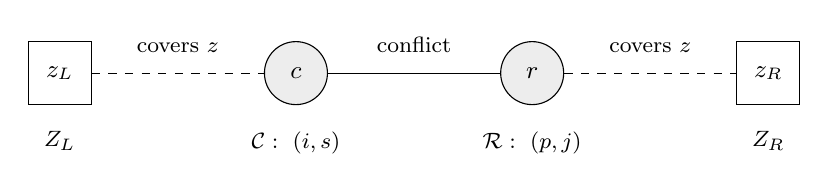
\begin{tikzpicture}[
  every node/.style={font=\small},
  original/.style={circle,draw,fill=black!7,minimum size=8mm,inner sep=1pt},
  copy/.style={rectangle,draw,minimum size=8mm,inner sep=3pt},
  edge label/.style={font=\footnotesize,above=4pt},
  family label/.style={font=\footnotesize,below=6pt}
]
 \node[copy] (zl) at (0,0) {$z_L$};
 \node[original] (c) at (3,0) {$c$};
 \node[original] (r) at (6,0) {$r$};
 \node[copy] (zr) at (9,0) {$z_R$};
 \draw[dashed] (zl) -- node[edge label] {covers $z$} (c);
 \draw (c) -- node[edge label] {conflict} (r);
 \draw[dashed] (r) -- node[edge label] {covers $z$} (zr);
 \node[family label] at (zl.south) {$Z_L$};
 \node[family label] at (c.south) {$\mathcal C:\ (i,s)$};
 \node[family label] at (r.south) {$\mathcal R:\ (p,j)$};
 \node[family label] at (zr.south) {$Z_R$};
\end{tikzpicture}
 \caption{The three edges forced by one conflict between $r=(p,j)$ and
 $c=(i,s)$, where $z=(i,j)$.  Different conflicts may share vertices and
 edges.}
 \label{fig:pruning}
\end{figure}

\emph{(A1) A conflict-free member is isolated in $\Gamma$.}
Suppose $(p,j)\in\mathcal R$ covers $(i,j)\in Z$, so $p\to i$.  A conflict
witnessing $(i,j)\in Z$ supplies $(i,s)\in\mathcal C$ with $s\to j$, and
this member conflicts with $(p,j)$.  The case of $\mathcal C$ is symmetric.

\emph{(A2) A small cover suffices.}
Let $K$ be a vertex cover of $\Gamma$ with $\abs K\le\abs Z+\abs H$ that
contains no isolated vertex.  Put $\mathcal R'=\mathcal R\setminus K$ and
$\mathcal C'=\mathcal C\setminus K$.  Every conflict is an edge with an
endpoint in $K$, so no conflict survives.  By (A1), conflict-free members
are retained.  Let $q$ be the number of points of $Z$ covered by no member
of $\mathcal R'\cup\mathcal C'$.  Each of the other $\abs Z-q$ points $z$ is
covered by a surviving member, which is adjacent to a copy of $z$ and is not
in $K$; so that copy lies in $K$.  Distinct points give distinct copies,
whence
\begin{equation}\label{eq:cover-charge}
 \abs{K\cap(\mathcal R\sqcup\mathcal C)}
 \leq \abs K-(\abs Z-q)\leq\abs H+q,
\end{equation}
which is \eqref{eq:pruning-bound}.  It remains to find $K$.

\medskip\noindent
\emph{Part B: a special maximum matching.}
Among all maximum matchings of $\Gamma$ choose one, $\mathcal M$, with the
fewest edges between $\mathcal R$ and $\mathcal C$.  Let $k$ be the number of
these edges, $\alpha$ the set of $\mathcal M$-edges between $\mathcal R$ and
$Z_R$, and $\beta$ those between $Z_L$ and $\mathcal C$.  With
$\ell=\abs\alpha$ and $t=\abs\beta$,
\[
 \abs{\mathcal M}=k+\ell+t.
\]
Let $R_\alpha\subseteq\mathcal R$ and $C_\beta\subseteq\mathcal C$ be the
sets of original endpoints of $\alpha$ and $\beta$.  The endpoints of the
$k$ edges between $\mathcal R$ and $\mathcal C$ lie outside
$R_\alpha\cup C_\beta$.

\emph{(B1) $\alpha$ is a maximum matching of the subgraph $\Gamma_\alpha$
induced on $\mathcal R\sqcup Z_R$, and $\beta$ of the subgraph
$\Gamma_\beta$ induced on $Z_L\sqcup\mathcal C$.}
Suppose $\Gamma_\alpha$ has a larger matching.  Its symmetric difference
with $\alpha$ contains an $\alpha$-augmenting path $\pi$ in $\Gamma_\alpha$,
from an $\alpha$-unmatched $r_0\in\mathcal R$ to an $\alpha$-unmatched
$z_R\in Z_R$.  Vertices of $Z_R$ have neighbours only in $\mathcal R$, so
their $\mathcal M$-edges lie in $\alpha$; hence $z_R$ is
$\mathcal M$-unmatched.  Each internal vertex of $\pi$ is matched in
$\mathcal M$ by an $\alpha$-edge of $\pi$.  If $r_0$ is
$\mathcal M$-unmatched, $\pi$ augments $\mathcal M$, contradicting
maximality.  Otherwise the $\mathcal M$-edge at $r_0$ is some $r_0c$ with
$c\in\mathcal C$.  Then $\pi$ is augmenting for
$\mathcal M\setminus\{r_0c\}$, and augmenting gives a matching of size
$\abs{\mathcal M}$ with $k-1$ edges between $\mathcal R$ and $\mathcal C$,
contradicting the choice of $\mathcal M$.  The argument for $\beta$ is the
same with the sides exchanged.

\medskip\noindent
\emph{Part C: four matrices with $NL=AB$.}
For each arrow $x\to y$ take two symbols $a_{xy}$ and $b_{xy}$; set
$a_{xy}=b_{xy}=0$ when $x\not\to y$.  For any real values of the symbols
define
\[
 \begin{array}{ccc}
 \R^{\mathcal R}&\xrightarrow{\ L\ }&\R^Z\\[3pt]
 {\scriptstyle B}\big\downarrow&&\big\downarrow{\scriptstyle N}\\[3pt]
 \R^H&\xrightarrow{\ A\ }&\R^{\mathcal C}
 \end{array}
\]
by (row index first, column index second)
\begin{equation}\label{eq:pruning-maps}
 \begin{aligned}
 L_{(i,j),(p,j)}&=a_{pi},&
 N_{(i,s),(i,j)}&=b_{sj},\\
 B_{(p,s),(p,j)}&=b_{sj},&
 A_{(i,s),(p,s)}&=a_{pi},
 \end{aligned}
\end{equation}
all entries not of a listed form being zero.  So $L$ and $A$ move the first
coordinate along $p\to i$ and fix the second, while $N$ and $B$ move the
second coordinate from $j$ to $s$ along $s\to j$ and fix the first.  In
particular $L_{z,r}\ne0$ only if $r$ covers $z$, and $N_{c,z}\ne0$ only if
$c$ covers $z$.

Fix a column $(p,j)\in\mathcal R$ and a row $(i,s)\in\mathcal C$.  In
$(NL)_{(i,s),(p,j)}=\sum_{z\in Z}N_{(i,s),z}L_{z,(p,j)}$ the only index $z$
that can contribute is $(i,j)$.  In $(AB)_{(i,s),(p,j)}$ the only index of
$H$ that can contribute is $(p,s)$.  If $(p,j)$ and $(i,s)$ conflict, then
$(i,j)\in Z$ and $(p,s)\in H$, and both entries equal $a_{pi}b_{sj}$.  If
they do not conflict, then $p\not\to i$ or $s\not\to j$, so
$a_{pi}b_{sj}=0$ and both entries vanish.  Hence
\begin{equation}\label{eq:pruning-commute}
 NL=AB.
\end{equation}

\medskip\noindent
\emph{Part D: three conditions that give the matching bound.}
Suppose real values are chosen with
\begin{equation}\label{eq:three-conditions}
 \rank L=\ell,\qquad \rank N=t,\qquad \dim\ker A\geq k.
\end{equation}
Then
\begin{equation}\label{eq:pruning-rank-bound}
 \abs H=\dim\ker A+\rank A
 \geq k+\rank(AB)=k+\rank(NL)
 \geq k+\ell+t-\abs Z .
\end{equation}
The steps are: rank--nullity for $A$; $\im(AB)\subseteq\im A$;
\eqref{eq:pruning-commute}; and
$\rank(NL)=\dim\im L-\dim(\im L\cap\ker N)\ge\ell-(\abs Z-t)$.
So \eqref{eq:three-conditions} implies
$\abs{\mathcal M}\le\abs Z+\abs H$.  Part E obtains the first two conditions
and Parts F--H the third.

\medskip\noindent
\emph{Part E: one real assignment for all rank conditions.}
For every arrow $p\to i$ define
\[
 J_p=\{j:(p,j)\in\mathcal R\},\qquad
 S_i=\{s:(i,s)\in\mathcal C\},\qquad
 W^{p,i}=(b_{sj})_{s\in S_i,\ j\in J_p},
\]
a matrix supported on
$\Omega^{p,i}=\{(s,j)\in S_i\times J_p:s\to j\}$.  Let $\rho^{p,i}$ be the
maximum rank of a real matrix supported on $\Omega^{p,i}$.

Regard the symbols $a_{xy},b_{xy}$ ($x\to y$) as indeterminates, so that
$L$, $N^{\mathsf T}$, $W^{p,i}$ have entries in the polynomial ring
$\R[a,b]$.  The idea is the classical link between generic rank and maximum
matchings \cite[Section~5, Theorem~1]{Edmonds1967}.  Because indeterminates
are shared between matrices, we argue directly.  Consider these finitely
many polynomials.
\begin{itemize}[leftmargin=*]
\item[(P1)] $\pi_\alpha$: the minor of $L$ on the columns $R_\alpha$ and the
rows $z$ with $z_R$ matched by $\alpha$.
\item[(P2)] $\pi_\beta$: the minor of $N^{\mathsf T}$ (columns indexed by
$\mathcal C$, rows by $Z$) on the columns $C_\beta$ and the rows $z$ with
$z_L$ matched by $\beta$.
\item[(P3)] For each arrow $p\to i$, a $\rho^{p,i}\times\rho^{p,i}$ minor
$\pi^{p,i}$ of $W^{p,i}$, chosen below.
\end{itemize}

\emph{(P1) is a nonzero polynomial.}  The entry of $L$ in row $(i,j')$ and
column $(p,j)$ vanishes unless $j'=j$, and $\alpha$ matches each $(p,j)$ to
a point with the same second coordinate.  Ordering rows and columns by
second coordinate, the submatrix is block diagonal with one \emph{square}
block per $j$, so $\pi_\alpha$ is $\pm$ the product of the block
determinants.  In the block for $j$, the entry in row $(i,j)$ and column
$(p,j)$ is the indeterminate $a_{pi}$ if $p\to i$ and $0$ otherwise, and
distinct positions carry distinct indeterminates.  So each permutation
contributing to the block determinant gives $\pm$ a squarefree monomial
that determines the permutation, and no two terms cancel.  The restriction
of $\alpha$ to the block is one such permutation.  Hence each block
determinant is nonzero.  An indeterminate may occur in several blocks, but
$\R[a,b]$ is an integral domain, so $\pi_\alpha\ne0$.

\emph{(P2) is a nonzero polynomial.}  The same argument applies:
$(N^{\mathsf T})_{(i,j),(i',s)}$ vanishes unless $i'=i$, the blocks are
indexed by the first coordinate $i$, and within a block distinct positions
carry distinct indeterminates $b_{sj}$.

\emph{(P3) can be chosen nonzero.}  Take a real matrix $W_0$ supported on
$\Omega^{p,i}$ of rank $\rho^{p,i}$, and a nonzero
$\rho^{p,i}\times\rho^{p,i}$ minor of $W_0$ (the empty minor if
$\rho^{p,i}=0$).  Let $\pi^{p,i}$ be the same minor of $W^{p,i}$.  The
entries of $W^{p,i}$ on $\Omega^{p,i}$ are distinct indeterminates, so
substituting the entries of $W_0$ is a legitimate evaluation of
$\pi^{p,i}$.  It gives a nonzero number, hence $\pi^{p,i}\ne0$.

\emph{One assignment.}  The product of $\pi_\alpha$, $\pi_\beta$ and all
$\pi^{p,i}$ is a nonzero element of $\R[a,b]$, again because $\R[a,b]$ is a
domain.  A nonzero real polynomial is nonzero at some real point (induction
on the number of variables: a nonzero one-variable polynomial has finitely
many roots).  Fix such a point once and for all.  From now on the symbols
are these real numbers, and every polynomial in (P1)--(P3) is nonzero at
them.  Consequences:
\begin{itemize}[leftmargin=*]
\item[(E1)] $\rank L=\ell$, and the columns $R_\alpha$ of $L$ form a basis
of $\im L$.  For the upper bound, a nonzero square minor of $L$ has a
nonzero term in its expansion.  That term selects, for the chosen columns
$r$, distinct rows $z$ with $L_{z,r}\ne0$, i.e.\ edges $rz_R$ of
$\Gamma_\alpha$; this is a matching of the size of the minor, which is at
most $\ell$ by (B1).  For the lower bound, $\pi_\alpha\ne0$ makes the $\ell$
columns $R_\alpha$ independent.
\item[(E2)] Likewise $\rank N=\rank N^{\mathsf T}=t$, and the columns
$C_\beta$ of $N^{\mathsf T}$ form a basis of $\im N^{\mathsf T}$.
\item[(E3)] Each $W^{p,i}$ has rank $\rho^{p,i}$: at least $\rho^{p,i}$
since $\pi^{p,i}\ne0$, at most $\rho^{p,i}$ since it is supported on
$\Omega^{p,i}$.  So $W^{p,i}$ has maximum rank among real matrices supported
on $\Omega^{p,i}$.
\end{itemize}

\medskip\noindent
\emph{Part F: lifts.}
Let $rc$ be an edge of $\mathcal M$ with $r\in\mathcal R$, $c\in\mathcal C$;
then $r\notin R_\alpha$ and $c\notin C_\beta$.  By (E1), $Le_r$ is a
combination of the columns $R_\alpha$ of $L$.  By (E2), $N^{\mathsf T}e_c$
is a combination of the columns $C_\beta$ of $N^{\mathsf T}$.  So there are
reals $\lambda^r_\rho,\mu^c_\gamma$ with
\begin{equation}\label{eq:pruning-lifts}
 u^r=e_r+\sum_{\rho\in R_\alpha}\lambda_\rho^r e_\rho\in\ker L,
 \qquad
 v^c=e_c+\sum_{\gamma\in C_\beta}\mu_\gamma^c e_\gamma
                 \in\ker N^{\mathsf T}.
\end{equation}
If $r,r'$ are left endpoints of two such edges, the $r'$-coordinate of $u^r$
is $1$ if $r'=r$ and $0$ otherwise.  Also $v^c_c=1$.

\medskip\noindent
\emph{Part G: the kernel restriction.}
We claim that
\begin{equation}\label{eq:conflict-kernel}
 u_{(p,j)}\,v_{(i,s)}=0
 \quad\text{for every conflict }((p,j),(i,s)),\ \text{every }
 u\in\ker B,\ \text{and every }v\in\ker N^{\mathsf T}.
\end{equation}
Fix such a conflict, $u$ and $v$.  Then $p\to i$, and we write $W=W^{p,i}$.

\emph{(G1) $x=(u_{(p,j')})_{j'\in J_p}$ lies in $\ker W$.}
The row of $Wx$ at $s'\in S_i$ is $\sum_{j'\in J_p}b_{s'j'}u_{(p,j')}$.
Suppose first that $s'\to j'$ for some $j'\in J_p$.  Then
$(p,j')\in\mathcal R$ and $(i,s')\in\mathcal C$ conflict (as $p\to i$), so
$(p,s')\in H$.  By \eqref{eq:pruning-maps} the nonzero entries of $B$ in
row $(p,s')$ sit in the columns $(p,j')$, $j'\in J_p$, with values
$b_{s'j'}$.  So the sum is the full $(p,s')$-coordinate of $Bu$, which is
$0$.  If instead there is no such $j'$, every coefficient $b_{s'j'}$ is $0$
by convention and the sum is trivially $0$; here $(p,s')$ need not belong
to $H$, and no coordinate of $Bu$ is used.

\emph{(G2) $y=(v_{(i,s')})_{s'\in S_i}$ lies in $\ker W^{\mathsf T}$.}
The entry of $W^{\mathsf T}y$ at $j'\in J_p$ is
$\sum_{s'\in S_i}b_{s'j'}v_{(i,s')}$.  If $s'\to j'$ for some $s'\in S_i$,
the same conflict gives $(i,j')\in Z$, and the sum is the full
$(i,j')$-coordinate of $N^{\mathsf T}v=0$.  Otherwise all coefficients
vanish.

\emph{(G3)} We have $(s,j)\in\Omega^{p,i}$, because $s\in S_i$, $j\in J_p$
and $s\to j$.  By (E3), Lemma~\ref{lem:kernel-support} applies to the fixed
real matrix $W$ and gives $x_jy_s=0$, which is \eqref{eq:conflict-kernel}.
The perturbation inside the proof of that lemma is only a comparison matrix
supported on $\Omega^{p,i}$; the fixed assignment is not changed.

\medskip\noindent
\emph{Part H: $\dim\ker A\ge k$.}
Let $rc$ be one of the $k$ edges of $\mathcal M$ between $\mathcal R$ and
$\mathcal C$.  It is a conflict, so \eqref{eq:conflict-kernel} with $v=v^c$
and $v^c_c=1$ shows that \emph{every} $u\in\ker B$ has $u_r=0$.  Now suppose
$\sum_r\theta_rBu^r=0$, the sum over the $k$ left endpoints.  Then
$u=\sum_r\theta_ru^r\in\ker B$, and its coordinate at each such endpoint
$r$ is $\theta_r$ by Part F; hence all $\theta_r=0$.  So the $k$ vectors
$Bu^r$ are linearly independent.  They lie in $\ker A$, since
$A(Bu^r)=NLu^r=0$ by \eqref{eq:pruning-commute} and
\eqref{eq:pruning-lifts}.  With (E1) and (E2), all three conditions in
\eqref{eq:three-conditions} hold, and \eqref{eq:pruning-rank-bound} gives
\[
 \abs{\mathcal M}=k+\ell+t\le\abs Z+\abs H .
\]

\medskip\noindent
\emph{Part I: from the matching to the cover.}
This is the standard argument for K\H{o}nig's theorem~\cite{konig1931}.
Starting from all $\mathcal M$-unmatched vertices of $\mathcal V_L$, follow
edges outside $\mathcal M$ from left to right and edges of $\mathcal M$ from
right to left.  Let $W_L,W_R$ be the sets of reached vertices on the two
sides.  No unmatched right vertex is reached, since the path to it would
augment $\mathcal M$.  The endpoints of a matched edge are both reached or
both unreached: a reached right endpoint leads to its mate, and a matched
left vertex can be reached only through its mate.  Put
\[
 K=(\mathcal V_L\setminus W_L)\cup W_R .
\]
$K$ is a cover: an edge from $W_L$ to $\mathcal V_R\setminus W_R$ can be
neither unmatched (it would be traversed) nor matched (its endpoints have
equal reachability).  $K$ contains exactly one endpoint of each matched
edge and no unmatched vertex, so
$\abs K=\abs{\mathcal M}\le\abs Z+\abs H$.  Isolated vertices are unmatched
and hence not in $K$.  By (A2) the lemma follows.
\end{proof}

\section{The extremal contradiction}\label{sec:incompatibility}

\begin{proposition}\label{prop:no-concavity}
There is no nonempty finite oriented graph $G$ in which every vertex has an
in-neighbor and whose one-step image operator
\[
 F(U)=\{y\in V(G):x\to y\text{ for some }x\in U\}
\]
satisfies
\begin{equation}\label{eq:impossible-concavity}
 \abs{U}+\abs{F^2(U)}<2\abs{F(U)}
 \qquad(\varnothing\ne U\subsetneq V(G)),
\end{equation}
where $F^2=F\circ F$.
\end{proposition}

\begin{proof}
\emph{Plan.}  Assume $G$ exists.  Choose an extremal compatible pair $(P,Q)$
(Steps 1--2).  Use \eqref{eq:impossible-concavity} to build larger families
$\mathcal R,\mathcal C$ (Steps 3--4).  Check the hypotheses needed to prune
them cheaply (Steps 5--6).  Prune, and beat the extremal value (Step 7).

\smallskip\noindent\emph{Step 1: coordinate images and compatibility.}
Put $X=V(G)$.  For $\mathcal S\subseteq X\times X$ define
\[
 \begin{aligned}
 F_1\mathcal S&=\{(i,j): (p,j)\in\mathcal S\text{ and }p\to i
                     \text{ for some }p\in X\},\\
 F_2\mathcal S&=\{(i,j): (i,s)\in\mathcal S\text{ and }s\to j
                     \text{ for some }s\in X\},
 \end{aligned}
\]
$F_1^2=F_1\circ F_1$, $F_2^2=F_2\circ F_2$, and
$\Delta=\{(v,v):v\in X\}$.  Call $P,Q\subseteq X\times X$ \emph{compatible}
if $F_1P\cap F_2Q=\varnothing$.  Unwinding the definitions, a point $(i,j)$
lies in $F_1P\cap F_2Q$ exactly when some $(p,j)\in P$ and $(i,s)\in Q$
satisfy $p\to i$ and $s\to j$.  So compatibility means that $P$ (as
$\mathcal R$) and $Q$ (as $\mathcal C$) have no conflict in the sense of
Lemma~\ref{lem:pruning}.  Likewise, $F_1P$ is the set of points covered by
a member of $P$, and $F_2Q$ the set covered by a member of $Q$.

\smallskip\noindent\emph{Step 2: the extremal pair.}
The pair $(\Delta,\Delta)$ is compatible: $(i,j)\in F_1\Delta$ means
$j\to i$ and $(i,j)\in F_2\Delta$ means $i\to j$, and both cannot hold in an
oriented graph.  As $X$ is finite, we may choose a compatible pair $(P,Q)$
with $\Delta\subseteq P\cap Q$ maximizing $M+d$, where
\[
 M=\abs{P}+\abs{Q},\qquad
 d=\abs{X}^2-\abs{F_1P}-\abs{F_2Q}.
\]
By compatibility, $d$ is the number of points outside $F_1P\cup F_2Q$.

\smallskip\noindent\emph{Step 3: applying \eqref{eq:impossible-concavity}
fibrewise.}
For $j\in X$ let $P_j=\{p:(p,j)\in P\}$ be the $j$-th column of $P$.  By
definition of $F_1$, the $j$-th column of $F_1P$ is $F(P_j)$, and that of
$F_1^2P$ is $F^2(P_j)$.

$P_j$ is nonempty since $j\in P_j$.  It is proper.  Indeed, positive
indegrees give $F(X)=X$, so $P_j=X$ would give
$X\times\{j\}\subseteq F_1P$.  Choose an in-neighbour $w$ of $j$; then
$(w,w)\in Q$ and $w\to j$ give $(w,j)\in F_2Q$, contradicting
compatibility.  Symmetrically, each row $Q_i=\{s:(i,s)\in Q\}$ contains
$i$.  If $Q_i=X$ then $\{i\}\times X\subseteq F_2Q$, while $w\to i$ and
$(w,w)\in P$ give $(i,w)\in F_1P$, again a contradiction.

Summing \eqref{eq:impossible-concavity} for $U=P_j$ over $j\in X$, and for
$U=Q_i$ over $i\in X$, gives
\begin{equation}\label{eq:strict-fiber-sums}
 \abs{P}+\abs{F_1^2P}<2\abs{F_1P},\qquad
 \abs{Q}+\abs{F_2^2Q}<2\abs{F_2Q}.
\end{equation}

\smallskip\noindent\emph{Step 4: the complement families.}  Define
\[
 \mathcal R=(X\times X)\setminus F_2^2Q,
 \qquad
 \mathcal C=(X\times X)\setminus F_1^2P.
\]
By \eqref{eq:strict-fiber-sums},
\begin{equation}\label{eq:complement-gain}
 \abs{\mathcal R}+\abs{\mathcal C}
 =2\abs{X}^2-\abs{F_2^2Q}-\abs{F_1^2P}
 >2\abs{X}^2+M-2\bigl(\abs{F_1P}+\abs{F_2Q}\bigr)
 =M+2d.
\end{equation}

\smallskip\noindent\emph{Step 5: the diagonal lies in both families and is
conflict-free.}
\emph{Membership.}  If $(v,v)\in F_2^2Q$, there is $s\to v$ with
$(v,s)\in F_2Q$; but $(s,s)\in P$ and $s\to v$ give $(v,s)\in F_1P$,
contradicting compatibility.  If $(v,v)\in F_1^2P$, there is $p\to v$ with
$(p,v)\in F_1P$; but $(p,p)\in Q$ and $p\to v$ give $(p,v)\in F_2Q$.

\emph{No conflicts.}  A conflict between $(v,v)\in\mathcal R$ and
$(i,s)\in\mathcal C$ means $v\to i$ and $s\to v$.  Then $(s,s)\in P$ gives
$(v,s)\in F_1P$ and $(i,s)\in F_1^2P$, contradicting $(i,s)\in\mathcal C$.
A conflict between $(p,j)\in\mathcal R$ and $(v,v)\in\mathcal C$ means
$p\to v$ and $v\to j$.  Then $(p,p)\in Q$ gives $(p,v)\in F_2Q$ and
$(p,j)\in F_2^2Q$, contradicting $(p,j)\in\mathcal R$.

\smallskip\noindent\emph{Step 6: $\abs H\le d$.}
Let $H,Z$ be the sets attached to $\mathcal R,\mathcal C$ in
Lemma~\ref{lem:pruning}.  We claim
\begin{equation}\label{eq:old-uncovered-bound}
 H\subseteq (X\times X)\setminus(F_1P\cup F_2Q),
 \qquad\text{hence}\qquad \abs{H}\le d .
\end{equation}
Take a conflict $(p,j)\in\mathcal R$, $(i,s)\in\mathcal C$ with $p\to i$ and
$s\to j$.  If $(p,s)\in F_1P$, then $p\to i$ puts $(i,s)$ in $F_1^2P$,
contradicting $(i,s)\in\mathcal C$.  If $(p,s)\in F_2Q$, then $s\to j$ puts
$(p,j)$ in $F_2^2Q$, contradicting $(p,j)\in\mathcal R$.

\smallskip\noindent\emph{Step 7: pruning and the contradiction.}
Lemma~\ref{lem:pruning} gives conflict-free $P'\subseteq\mathcal R$ and
$Q'\subseteq\mathcal C$ retaining all conflict-free members.  By Step 5,
$\Delta\subseteq P'\cap Q'$.  By Step 1, $(P',Q')$ is compatible.  So
$(P',Q')$ competes in the maximization of Step 2, with
\[
 d'=\abs{X}^2-\abs{F_1P'}-\abs{F_2Q'}
\]
equal to the number of points of $X\times X$ outside $F_1P'\cup F_2Q'$.  By
Step 1, a point is covered by a member of $P'\cup Q'$ exactly when it lies
in $F_1P'\cup F_2Q'$.  So the uncovered points of $Z$ in
\eqref{eq:pruning-bound} are among these $d'$ points.  With
\eqref{eq:old-uncovered-bound}, at most $d+d'$ members were deleted, and
\eqref{eq:complement-gain} gives
\[
 \abs{P'}+\abs{Q'}+d'
 \ge \abs{\mathcal R}+\abs{\mathcal C}-(d+d')+d'
 >M+2d-(d+d')+d'=M+d.
\]
This contradicts the choice of $(P,Q)$.
\end{proof}

\begin{proof}[Proof of Theorem~\ref{thm:main}]
If the theorem were false, Proposition~\ref{prop:counterexample-reduction}
would give a nonempty finite oriented graph with positive indegrees
satisfying~\eqref{eq:impossible-concavity} for every nonempty proper vertex
set.  Proposition~\ref{prop:no-concavity} excludes this.
\end{proof}

\section{Weighted consequences}\label{sec:weighted-consequences}

The corollary applies Theorem~\ref{thm:main} through Seacrest's established
equivalences~\cite{Seacrest2015}, which are not new here.  Part (iii) is
taken from that reference without re-derivation.  Parts (i) and (ii) are
then checked directly.

\begin{corollary}[Weighted second-neighborhood forms]\label{cor:weighted-forms}
Let \(D\) be a nonempty finite oriented graph with arc set \(A(D)\).  For
\(\eta:V(D)\to[0,\infty)\) write \(\eta(S)=\sum_{x\in S}\eta(x)\).
\begin{enumerate}[label=\textup{(\roman*)}]
\item For every vertex weighting \(\eta:V(D)\to[0,\infty)\) there is a
vertex \(v\) with
\(\eta(N_1^+(v))\leq\eta(N_2^+(v))\).

\item There is a vertex weighting \(\eta:V(D)\to[0,\infty)\) with
\(\sum_{x}\eta(x)=1\) such that
\(\eta(N_1^+(v))\leq\eta(N_2^+(v))\) for every \(v\in V(D)\).
Some entries of $\eta$ may be zero.

\item For every arc weighting \(w:A(D)\to[0,\infty)\), set \(w(vs)=0\) when
\(vs\notin A(D)\), and for \(v,s\in V(D)\) put
\[
 \beta_v^w(s)=\max\Bigl(\{0\}\cup
 \{w(us)-w(vs):u\in V(D),\ v\to u\to s\}\Bigr).
\]
Then there is a vertex \(v\) with
\[
 \sum_{s\in V(D)}\beta_v^w(s)
 \geq \sum_{u\in N_1^+(v)}w(vu).
\]
Here $w(vs)$ enters only as a number.  Whether $v\to u\to s$ is a path is
decided by the arcs of $D$: an arc of weight zero is still an arc, and
$\beta_v^w(s)=0$ if there is no such path.
\end{enumerate}
\end{corollary}

\begin{proof}
\textup{(iii)} According to the source, Seacrest's
Proposition~2~\cite{Seacrest2015} proves that his arc-weighted Conjecture~4,
which is statement \textup{(iii)} for all nonempty finite oriented graphs,
is equivalent to the unweighted conjecture.  Theorem~\ref{thm:main}
therefore gives \textup{(iii)}.

\textup{(i)} Apply \textup{(iii)} with $w(us)=\eta(s)$ on every arc
$u\to s$.  Fix $v,s$.  If $v\to s$, every eligible difference is
$\eta(s)-\eta(s)=0$, so $\beta_v^w(s)=0$.  If $s\in N_2^+(v)$, then
$w(vs)=0$ and a path $v\to u\to s$ exists, so $\beta_v^w(s)=\eta(s)$.  In
all other cases (including $s=v$, by orientation) there is no path
$v\to u\to s$ and $\beta_v^w(s)=0$.  So the two sides of \textup{(iii)} are
$\eta(N_2^+(v))$ and $\eta(N_1^+(v))$.  This is the specialization noted
after Seacrest's Proposition~2.

\textup{(ii)} Let $\Phi_D$ be the $V(D)\times V(D)$ matrix with entry $1$ at
$(v,s)$ when $s\in N_2^+(v)$, $-1$ when $s\in N_1^+(v)$, and $0$ otherwise.
Then $(\Phi_D\eta)_v=\eta(N_2^+(v))-\eta(N_1^+(v))$.  Let $\overleftarrow D$
be $D$ with all arcs reversed.  Since $s$ is an exact second out-neighbour
of $v$ in $\overleftarrow D$ exactly when $v\in N_2^+(s)$ in $D$, and
similarly for first neighbours,
$\Phi_{\overleftarrow D}=\Phi_D^{\mathsf T}$.  The source cites Seacrest's
Theorem~1, which applies Farkas' lemma, for the following alternative: for a
real matrix $\Phi$, either (a) some nonzero $\eta\ge0$ has $\Phi\eta\ge0$,
or (b) some $\xi\ge0$ has $\Phi^{\mathsf T}\xi<0$ in every coordinate.  One
way to see it: by the minimax theorem,
$\max_\eta\min_v(\Phi\eta)_v=\min_\xi\max_s(\Phi^{\mathsf T}\xi)_s$ over
probability vectors; (a) holds if this value is $\ge0$ and (b) if it is
$<0$.  For $\Phi=\Phi_D$, alternative (b) says
$\xi(N_2^+(v))<\xi(N_1^+(v))$ for every vertex $v$ of $\overleftarrow D$,
contradicting \textup{(i)} for the oriented graph $\overleftarrow D$.  So
(a) holds; divide $\eta$ by its total weight.
\end{proof}

\section{Directed-cycle consequences}\label{sec:directed-cycle-consequences}

In an oriented graph with no directed triangle, every exact second
out-neighbour is a non-neighbour.  Part (i) below is the oriented-graph form
of Thomass\'e's non-neighbor statement recorded by
Sullivan~\cite[Conjecture~6.12]{Sullivan2006}.  Part (ii) is noted in
\cite[Section~3]{Sullivan2006}.  Part (iii) is the girth-four lower bound in
the Behzad--Chartrand--Wall minimum-order
conjecture~\cite{BehzadChartrandWall1970}, also recorded in
\cite[Section~4]{Sullivan2006}.

\begin{corollary}[Non-neighbors and directed cycles]\label{cor:directed-cycle-consequences}
Let \(D\) be a nonempty finite oriented graph of order \(n\).  For
\(v\in V(D)\), write
\[
 N_1^-(v)=\{u:u\to v\},\qquad
 d^\pm(v)=\abs{N_1^\pm(v)},\qquad
 \delta^\pm(D)=\min_{x\in V(D)}d^\pm(x),
\]
and let the set of non-neighbors of \(v\), excluding \(v\) itself, be
\[
 \overline N(v)=V(D)\setminus
 \bigl(\{v\}\cup N_1^+(v)\cup N_1^-(v)\bigr).
\]
\begin{enumerate}[label=\textup{(\roman*)}]
\item If \(D\) has no directed \(3\)-cycle, then some vertex \(v\) satisfies
\[
 d^+(v)\leq\abs{\overline N(v)},\qquad
 n-1\geq 2d^+(v)+d^-(v).
\]
\item If \(\delta^+(D)\geq n/3\) and \(\delta^-(D)\geq n/3\), then \(D\)
contains a directed \(3\)-cycle.
\item If \(r\geq1\) is an integer, \(d^+(v)=d^-(v)=r\) for every vertex,
and \(D\) has directed girth exactly four, then \(n\geq3r+1\).
\end{enumerate}
Here directed girth is the length of a shortest directed cycle.
\end{corollary}

\begin{proof}
\textup{(i)} Suppose \(D\) has no directed \(3\)-cycle, and let
\(w\in N_2^+(v)\) with a path \(v\to u\to w\).  By definition \(w\ne v\) and
\(w\notin N_1^+(v)\).  Also \(w\notin N_1^-(v)\), since \(w\to v\) would
close a directed \(3\)-cycle.  Thus \(N_2^+(v)\subseteq\overline N(v)\) for
every \(v\), and Theorem~\ref{thm:main} gives a vertex with
\(d^+(v)\leq\abs{N_2^+(v)}\leq\abs{\overline N(v)}\).  As \(D\) is oriented,
\(N_1^+(v)\) and \(N_1^-(v)\) are disjoint, so
\[
 n-1=d^+(v)+d^-(v)+\abs{\overline N(v)}
 \geq 2d^+(v)+d^-(v).
\]

\textup{(ii)} Without a directed \(3\)-cycle, \textup{(i)} would give
\(n-1\geq2\delta^+(D)+\delta^-(D)\geq n\), which is absurd.

\textup{(iii)} Directed girth four excludes directed \(3\)-cycles, and
\textup{(i)} with all degrees equal to \(r\) reads \(n-1\geq3r\).
\end{proof}

\section{Verification checklist}\label{sec:checklist}

No step of the rewrite is marked unverified.  A sceptical reader should
check these load-bearing points first.
\begin{enumerate}[leftmargin=*]
\item \emph{Lemma~\ref{lem:subset-deficit}, Steps 6 and 8.}  The inclusion
$N_{2,D_T}^+(v)\subseteq(N_{2,D}^+(v)\setminus C)\cup(Q\cap F(T))$ and the
\emph{exact} identity $g(T\cup Q)-g(T)=\abs C-\abs{Q\cap F(T)}$.  Together
with $d_2<d_1$ they give the strict increment
\eqref{eq:deficit-increment}.
\item \emph{Lemma~\ref{lem:blowup}, Steps 5--7.}  The upper bound for
$\abs{F_G^2(U)}$, the identity
$\abs{H_0}-2\abs{F(S)}+\abs{S\cap F(S)}
=\abs{F^2(S)\setminus F(S)}-\abs{F(S)\setminus S}$, and the separate
treatment of $S=V(D)$.
\item \emph{Lemma~\ref{lem:pruning}, Part A.}  Inequality
\eqref{eq:cover-charge}: every covered point of $Z$ forces a copy into the
cover.  This is where the ``uncovered'' term of \eqref{eq:pruning-bound}
arises.
\item \emph{Lemma~\ref{lem:pruning}, Parts C--D.}  The identity $NL=AB$
\eqref{eq:pruning-commute}, checked entrywise, and the chain
\eqref{eq:pruning-rank-bound}.
\item \emph{Lemma~\ref{lem:pruning}, Part E.}  Each of (P1)--(P3) is a
nonzero polynomial despite shared indeterminates, and one real point makes
them all nonzero.  The bound $\rank L\le\ell$ uses (B1).
\item \emph{Lemma~\ref{lem:pruning}, Parts G--H.}  In (G1)--(G2) each sum is
either a full coordinate of $Bu$ or $N^{\mathsf T}v$, or has all
coefficients zero.  Lemma~\ref{lem:kernel-support} then gives
\eqref{eq:conflict-kernel}, which forces the $Bu^r$ to be independent.
\item \emph{Proposition~\ref{prop:no-concavity}, Steps 5--7.}  The diagonal
members are conflict-free (so they survive), $\abs H\le d$
\eqref{eq:old-uncovered-bound}, the uncovered points of $Z$ number at most
$d'$, and the final arithmetic $M+2d-(d+d')+d'=M+d$.
\item \emph{External inputs.}  Theorem~\ref{thm:main} uses no cited result
beyond standard matching theory.  Corollary~\ref{cor:weighted-forms}(iii)
rests entirely on Seacrest's Proposition~2~\cite{Seacrest2015}, quoted as
reported by the source and not re-derived here; compare the definition of
$\beta_v^w$ with that reference.
\end{enumerate}

\bibliographystyle{plain}
\bibliography{references}
\end{document}
